\subsection{Change of base field}

Let N be a Galois extension of K and \(\Gamma\) the Galois group of N over K; further let \(N'\) be a Galois extension of \(K'\) with Galois group \(\Gamma'\) . We shall identify K (resp. \(K'\) ) with its image in N (resp. \(N'\) ). Let u be a homomorphism of K into \(K'\) and v a homomorphism of N into \(N'\) whose restriction to K equals u (cf.

Fig. 1). Let \(\sigma \in \Gamma'\) ; since \(u(\mathbf{K}) \subset \mathbf{K}'\) , \(\sigma\) is a \(u(\mathbf{K})\) -automorphism of \(\mathbf{N}'\) ; moreover \(v(\mathbf{N})\) is a Galois extension of \(u(\mathbf{K})\) , hence \(\sigma\) induces a \(u(\mathbf{K})\) -automorphism of \(v(\mathbf{N})\) (V, p.~55, Remark 1). In other words, for every \(\sigma \in \Gamma'\) there exists a unique element \(v^*(\sigma)\) of \(\Gamma\) such that

\[
\boldsymbol {v} \circ \boldsymbol {v} ^ {*} (\sigma) = \sigma \circ \boldsymbol {v}.\tag{8}
\]

\pandocbounded{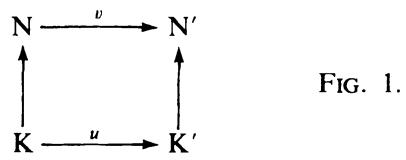
\includegraphics[keepaspectratio]{images/part002_8bfcf433.jpg}}

The mapping \(v^*\) is a homomorphism of \(\operatorname{Gal}(\mathbf{N}' / \mathbf{K}')\) into \(\operatorname{Gal}(\mathbf{N} / \mathbf{K})\) . For every \(x \in \mathbf{N}\) , the mapping \(\sigma \mapsto v^*(\sigma)(x) = v^{-1}(\sigma(v(x)))\) of \(\Gamma'\) into the discrete space \(\mathbf{N}\) is continuous, so \(v^*\) is continuous.

Three particular cases are of importance :

\begin{enumerate}
\def\labelenumi{\alph{enumi})}
\tightlist
\item
  If F is a Galois extension of K and E a subextension of F, we know (V, p.~67, Lemma 1) that F is a Galois extension of E. Let us apply what has been said to the case where N = F, \(K' = E\) , \(N' = F\) and \(v = Id_{F}\) . Then \(v^{*}\) is merely the canonical injection
\end{enumerate}

\[
j: \operatorname{Gal} (\mathrm{F} / \mathrm{E}) \rightarrow \operatorname{Gal} (\mathrm{F} / \mathrm{K}).
\]

This is sometimes called the inflation homomorphism.

\begin{enumerate}
\def\labelenumi{\alph{enumi})}
\setcounter{enumi}{1}
\tightlist
\item
  Suppose that in addition E is Galois over K. Let us apply what has been said to the case where N = E, \(K' = K\) , \(N' = F\) and v is the canonical injection of E into F. Then \(v^{*}\) is just the restriction homomorphism
\end{enumerate}

\[
\pi : \operatorname{Gal} (\mathrm{F} / \mathrm{K}) \rightarrow \operatorname{Gal} (\mathrm{E} / \mathrm{K}).
\]

We know (V, p.~60, Prop. 3) that \(\pi\) is surjective, with kernel \(\operatorname{Gal}(\mathrm{F} / \mathrm{E})\) and that by taking quotients it defines a topological group isomorphism of \(\operatorname{Gal}(\mathrm{F} / \mathrm{K}) / \operatorname{Gal}(\mathrm{F} / \mathrm{E})\) onto \(\operatorname{Gal}(\mathrm{E} / \mathrm{K})\) (V, p.~68, Cor. 4).

\begin{enumerate}
\def\labelenumi{\alph{enumi})}
\setcounter{enumi}{2}
\tightlist
\item
  Suppose that \(v^{-1}(\mathbf{K}') = \mathbf{K}\) and \(\mathbf{N}' = \mathbf{K}'(v(\mathbf{N}))\) ; let us show that the homomorphism
\end{enumerate}

\[
v ^ {*}: \operatorname{Gal} \left(\mathrm{N} ^ {\prime} / \mathrm{K} ^ {\prime}\right)\rightarrow \operatorname{Gal} (\mathrm{N} / \mathrm{K}),
\]

is a topological group isomorphism, sometimes called translation. For the group \(\operatorname{Gal}(N'/K')\) is compact, the group \(\operatorname{Gal}(N/K)\) is separated and \(v^{*}\) is continuous; so it is enough (Gen.~Top., I, p.~87, Cor. 2) to prove that \(v^{*}\) is bijective. Now every element \(\sigma\) of the kernel of \(v^{*}\) is an automorphism of \(N'\) which induces the identity on \(K'\) and on \(v(N)\) , hence \(\sigma = \varepsilon\) because \(\mathrm{N}' = \mathrm{K}'(v(N))\) ; it follows that \(v^{*}\) is injective. Further, the image of \(v^{*}\) is a closed subgroup \(\Delta\) of \(\operatorname{Gal}(N/K)\) .

(Gen.~Top., I, p.~81, ibid.) and the field of invariants of \(\Delta\) is equal to \(v^{-1}(\mathbf{K}') = \mathbf{K}\) ; therefore we have \(\Delta = \operatorname{Gal}(\mathbf{N}/\mathbf{K})\) (V, p.~67, Th. 4) and so \(v^{*}\) is surjective.

The general case may be reduced to the preceding ones by composition. To begin with we note that \(\mathrm{K}^{\prime}(v(\mathrm{N}))\) is the field of invariants in \(N^{\prime}\) of the kernel \(\Delta\) of \(v^{*}\) ; since \(\Delta\) is a normal subgroup of \(\operatorname{Gal}(\mathrm{N}^{\prime}/\mathrm{K}^{\prime})\) , the extension \(\mathrm{K}^{\prime}(v(\mathrm{N}))\) of \(K^{\prime}\) is Galois (V, p.~68, Cor. 4). Thus \(v^{*}\) is composed of the homomorphisms

\[
\operatorname{Gal} \left(\mathrm{N} ^ {\prime} / \mathrm{K} ^ {\prime}\right)\rightarrow \operatorname{Gal} \left(\mathrm{K} ^ {\prime} (v (\mathrm{N})) / \mathrm{K} ^ {\prime}\right) \stackrel {{\psi}} {{\rightarrow}} \operatorname{Gal} \left(\mathrm{N} / v ^ {- 1} \left(\mathrm{K} ^ {\prime}\right)\right) \stackrel {{j}} {{\rightarrow}} \operatorname{Gal} (\mathrm{N} / \mathrm{K});
\]

in this sequence \(\pi\) is the restriction homomorphism associated with the triple \(\mathbf{K}' \subset \mathbf{K}'(v(\mathbf{N})) \subset \mathbf{N}'\) , \(\psi\) is the translation isomorphism associated with the central square of the diagram (Fig. 2) and \(j\) is the inflation homomorphism associated with the triple \(\mathbf{K} \subset v^{-1}(\mathbf{K}') \subset \mathbf{N}\) .

The next theorem gives more detailed information about the structure of translation isomorphisms.

\[
\begin{array}{c}\mathbf {N} \rightarrow \mathbf {K} ^ {\prime} (v (\mathbf {N})) \rightarrow \mathbf {N} ^ {\prime}\\\uparrow \quad \uparrow\\\mathbf {K} \rightarrow v ^ {- 1} (\mathbf {K} ^ {\prime}) \rightarrow \mathbf {K} ^ {\prime}\end{array}\tag {FIG.2.}
\]

THEOREM 5. --- Let N' be an extension of K generated by two subextensions K' and N. Suppose that N is Galois over K, with Galois group Γ and that K' ∩ N = K. Then the extension N' of K' is Galois and the canonical homomorphism φ of K' ⊗K N into N' is an isomorphism. Let σ ∈ Gal(N/K) and let σ' be the element of Gal(N'/K') which corresponds to it under the translation isomorphism; then we have σ'∘φ = φ∘(Id\_\{K'\} ⊗σ).

We have \(N' = K'(N)\) and N is algebraic and separable over K; hence (V, p.~42, Prop. 10), the extension \(N'\) of \(K'\) is algebraic and separable. By Cor. 4 of V, p.~54 the extension \(N'\) of \(K'\) is quasi-Galois. Therefore the extension \(N'\) of \(K'\) is Galois. By c) above the mapping \(\sigma \mapsto \sigma | N\) is an homomorphism \(\lambda\) of \(\operatorname{Gal}(N'/K')\) onto \(\operatorname{Gal}(N/K)\) .

We have \(N = K'\) {[}N{]} because N is algebraic over K (V, p.~18, Cor. 1), hence \(\varphi\) is surjective. If \(\sigma\) belongs to \(\operatorname{Gal}(N/K)\) , we have

\[
\lambda^ {- 1} (\sigma) \circ \varphi = \varphi \circ \left(\operatorname{Id} _ {\mathrm{K} ^ {\prime}} \otimes \sigma\right).\tag{9}
\]

Therefore the kernel of \(\varphi\) is stable under the mappings \(\mathrm{Id}_{\mathbf{K}'} \otimes \sigma\) , hence of the form \(\mathbf{K}' \otimes_{\mathbf{K}} \mathbf{N}_0\) with \(\mathbf{N}_0 \subset \mathbf{N}\) (V, p.~63, Cor.). For \(x\) in \(\mathbf{N}_0\) we have \(x = \varphi(1 \otimes x) = 0\) , hence \(\mathbf{N}_0 = 0\) and so \(\varphi\) is injective.

COROLLARY 1. --- Let E' be a subfield of N' containing K'. There exists a unique subfield E of N containing K and such that E' = K'(E). We have E = E' ∩ N.

Put \(E = E' \cap N\) , then \(E' \supset K'(E)\) . Now put \(\Gamma = \text{Gal}(N/K)\) and \(\Delta = \text{Gal}(N/E)\) , and define \(\Gamma'\) and \(\Delta'\) similarly. The mapping \(\lambda : \sigma \mapsto \sigma | N\) is an isomorphism of \(\Gamma'\) onto \(\Gamma\) and also of \(\Delta'\) onto \(\Delta\) ; in other words, \(\Delta'\) consists of those \(\sigma \in \Gamma'\) for which \(\lambda(\sigma)\) belongs to \(\Delta\) . If \(\sigma \in \Gamma'\) leaves the elements of \(K'(E)\) fixed, we have \(\lambda(\sigma) \in \Delta\) , whence \(\sigma \in \Delta'\) and \(\sigma\) leaves the elements of \(E'\) fixed; by Cor. 1 of V, p.~68 we thus have \(K'(E) \supset E'\) .

We have proved the equality \(E' = K'(E)\) , whence \(\varphi^{-1}(E') = K' \otimes_{K} E\) . If F is a subfield of N containing K and such that \(E' = K'(F)\) , we have likewise \(\varphi^{-1}(E') = K' \otimes_{K} F\) , whence F = E.

COROLLARY 2. --- Let N be a Galois extension of K. Suppose that the Galois group \(\Gamma\) of N over K is the direct product of two closed subgroups \(\Gamma_1\) and \(\Gamma_2\) and denote by \(E_i\) the field of invariants of \(\Gamma_i\) for \(i = 1, 2\) . Then the canonical homomorphism of \(E_1 \otimes_K E_2\) into N is an isomorphism.

We have \(E_{1} \cap E_{2} = K\) and \(N = K(E_{1} \cup E_{2})\) by Cor. 6 (V, p.~69), and so it is enough to apply Theorem 5.

Remark. --- Let K and \(K'\) be two fields and u a homomorphism of K into \(K'\) . Let \(K_s\) (resp. \(K_s'\) ) be a separable closure (V, p.~45, Prop. 14) of K (resp. \(K'\) ) and \(\Pi\) (resp. \(\Pi'\) ) the Galois group of \(K_s\) over K (resp. \(K_s'\) over \(K'\) ). Since \(K_s\) is a separable algebraic extension of K and the extension ( \(K_s'\) , u) of K is separably closed, there exists (V, p.~45, Cor.) a homomorphism v of \(K_s\) into \(K_s'\) extending u. From v we obtain a continuous homomorphism \(v^*\) of \(\Pi'\) into \(\Pi\) . Let \(v_1\) be another extension of u; since \(K_s\) is a quasi-Galois extension of K, there exists an element \(\sigma_0\) of \(\Pi\) such that \(v_1 = v \circ \sigma_0\) . We conclude that \(v_1^*(\tau) = \sigma_0^{-1} v^*(\tau) \sigma_0\) for all \(\tau \in \Pi\) .

